\chapter{Theory}
\label{cha:theory}

% This chapter describes the static Android Package Kit (APK) features that are used for training the Naive Bayes (NB), Support Vector Machine (SVM), Random Forest (RF) and Convolutional Neural Network (CNN) classifiers implemented in this work.
% The theory behind each classifier is also briefly discussed.
% Lastly, the concept of exploratory data analysis is explained.
% Key aspects and various techniques are briefly explained and highlighted.

% \section{Static APK Features}

% Android applications can formally be represented as feature vectors $X_i$ of $D$-dimensional features $X_i = (x_1, ..., x_D)$.
% $N$ Android applications can thus be mathematically represented as a set $X$ of feature vectors, $X = (X_1, ..., X_N)$.

% In this work, each application is represented by its static APK features.
% An \texttt{.apk} file contains the code files of the application, the \texttt{AndroidManifest.xml} file, and the resources of the application (e.g., images).
% The static APK features will, in this work, mainly consist of information gathered from the permission list specified in the \texttt{AndroidManifest.xml} file.
% The features are provided by F-Secure\footnote{https://www.f-secure.com/en/f-secure}.
% A label $y_i = C_k$ (either malicious $k = 1$ or benign $k = 0$) has been manually set for each feature vector in the data set.

% \section{Naive Bayes}
% \label{sec:naive-bayes}
% The Naive Bayes (NB) classifier makes the assumption that all features are independent (Eq. \ref{eq:independence}) \cite{Lewis1998}.
% It uses conditional probability (Eq. \ref{eq:cond-prob}) together with Bayes' theorem (Eq. \ref{eq:bayes}) to create a probability distribution.
% For the classification of Android APKs, the probability distribution represents the probability for the vector $X_i$ to be classified as malicious ($y_i = C_1$) or benign ($y_i = C_0$).
% \(p(C_0|X_i)\) is thus the probability that the $i$-th vector is classified as benign.

% \begin{equation} \label{eq:independence}
%   p(x_1, ..., x_D) = \prod_{d=1}^{D} p(x_d)
% \end{equation}

% \begin{equation} \label{eq:chain-rule}
%   p(x_1, ..., x_D) = p(x_1|x_2, ..., x_D)p(x_2,...,x_D)
% \end{equation}

% \begin{equation} \label{eq:cond-prob}
%   p(C_k|x_1, ..., x_D) = p(C_k|X_i)
% \end{equation}

% \begin{equation} \label{eq:bayes}
%   p(C_k|X_i) = \frac{p(X_i|C_k) p(C_k)}{p(X_i)}
% \end{equation}

% The NB classifier can, together with the chain rule (Eq. \ref{eq:chain-rule}) and the independent assumption, be written as Eq. \ref{eq:naive-bayes}.

% \begin{equation} \label{eq:naive-bayes}
%   p(C_k|X_i) \propto p(C_k)\prod_{d=1}^{D} p(x_d|C_k)
% \end{equation}

% Classification with NB can now be done by choosing the label $y_t$ with maximum probability for a new input vector $X_t$ (Eq. \ref{eq:naive-bayes-max}.

% \begin{equation} \label{eq:naive-bayes-max}
%   y_t = \argmax_{k\in\{0, 1\}}p(C_k|X_t)
% \end{equation}

% The problem with NB classification is that features are usually not independent \cite{Lewis1998}.
% In order to improve the accuracy of the traditional NB classifiers, an improved NB classifier has been adapted and used with success in the industry \cite{Shang2017}, see Section \ref{sec:WNBC}.

% \section{Support Vector Machines}

% Support Vector Machines (SVMs) use a decision boundary for classifying data points.
% In the general case, the decision boundary is decided by maximising the margin \cite{Bishop2006}. 
% The margin is the distance between the decision boundary and all data points \cite{Cortes1995}.
% The margin can be expressed by only using a set of the closest data points, which means that the formulation of the SVM is generally sparse \cite{Bishop2006}.
% The points in this set are aptly named Support Vectors.

% The decision boundary is defined to be the hyperplane $w^Tx - b = 0$.
% The margin hyperplanes for the two classes are thus $w^Tx - b = 1$ and $w^Tx -b = -1$, respectively.
% A new data point $x_i$ is then classified by looking at the sign (positive or negative) of $w^T x_i - b$. 

% Hard margins are used when the data is assumed to be linearly separable.
% Linearly separable data means that all the data points can be correctly classified using a linear decision boundary.
% Hard margins have no flexibility to misclassify data points \cite{Bishop2006}.

% Soft margins can be used in the case where the data is not linearly separable.
% The soft margins allow for some \emph{slack} to exist, meaning some points will be wrongly classified \cite{Cortes1995}.
% This introduced slack would, if not controlled, allow the SVM to misclassify every single point in order to maximise the margin \cite{Bishop2006}. 
% The slack can be controlled using regularisation \cite{Bishop2006}.
% Regularisation is the concept of minimising a loss function which penalises misclassifications with respect to a given parameter $\lambda$.
% The regularisation parameter $\lambda$ can be seen as a parameter controlling the size of the margin and the size of the loss function (the number of misclassified data points).

% SVMs can also use \emph{kernels} to transform the input space into a generally higher dimensional space \cite{Bishop2006}.
% Figure \ref{fig:svm-rbf} illustrates an example using a radial basis function (RBF) kernel to transform the data points.
% The decision boundary is still linear in the transformed kernel space, but in the original input space it is nonlinear, as shown in Figure \ref{fig:svm-rbf}.
% The nonlinear decision boundary in the input space allows the SVM to correctly classify data points that are not linearly separable in the input space \cite{Bishop2006}.

% AntiMalDroid by Zhao et al. \cite{Zhao2011} is a SVM-based framework developed for the task of detecting Android malware.
% It is briefly described and discussed in Section \ref{sec:AntiMalDroid}.

% \begin{figure}
%   \centering
%     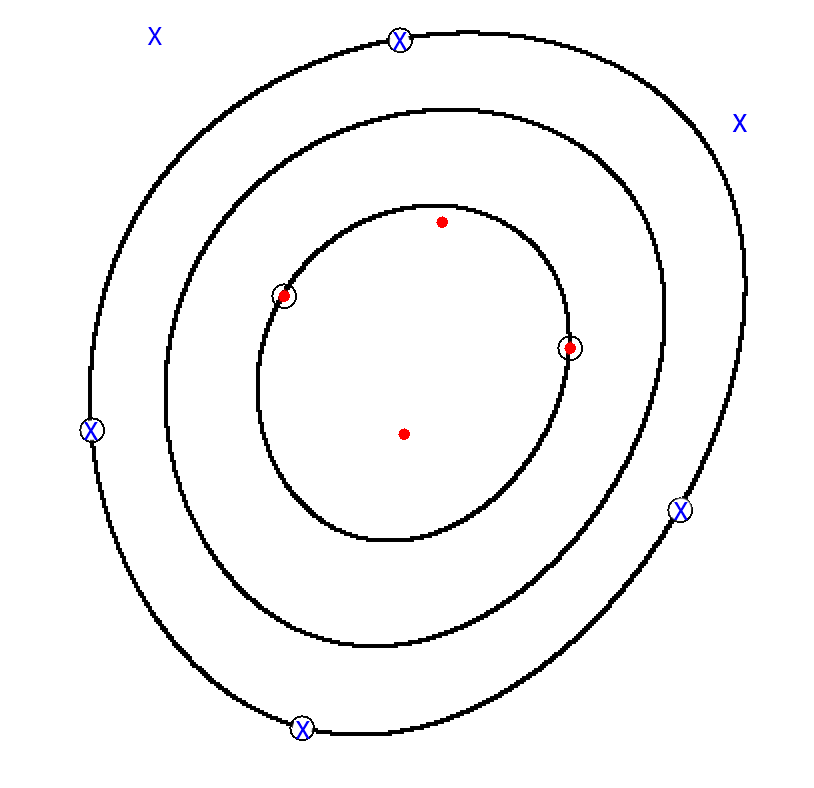
\includegraphics[width=0.75\textwidth]{figures/SVM_RBF_Circular}
%   \caption{A SVM using the RBF kernel.
%   It creates a decision boundary between the two classes that can be used to classify new points.
%   The decision boundary is the middle black line, surrounded by the visual margin.
%   The points with circles are the support vectors which define the margin and decision boundary.
%   For this data set, the RBF kernel creates a nonlinear decision boundary which correctly classifies all data points.}
%   \label{fig:svm-rbf}
% \end{figure}

% \newpage
% \section{Random Forest}
% Random Forest (RF) classifiers use multiple decision trees for classification.
% Decision trees classify data points by traversing the trained tree until a leaf is reached.
% The leaf contains the label that shall be assigned to the data point.
% An example of a simple decision tree would be to look at $x_1$ in the feature vector and split the tree if $x_1 < a$, for some number $a$.
% Then the decision would take into consideration $x_2$, until a leaf is reached.
% Dimensional splits of a feature vector is denoted a \textit{subspace} of the feature vector.

% Instead of only using one decision tree, trained on a certain subspace of feature vectors, the RF algorithm trains multiple decision trees \cite{Breiman2001, Ho1995} using random subspaces \cite{Ho1998}.
% In order to combine the classifications of all the trained trees, a \textit{discriminant function} is used.
% The discriminant function can be seen as every tree voting on the label of the sample \cite{Breiman2001}.
% Averaging the output of the decision trees in a RF classifier has been proven to reduce the variance of individual decision trees \cite{Breiman2001}.
% The averaging can be seen as removing the correlation between the decision trees \cite{Ho1998}.

% In \cite{Alam2013}, Alam et al. state a few key observations about using the Random Forest classifier for classifying APKs:
% \begin{itemize}
%     \item The result generally improves with the increased number of trees used.
%     \item The depth of the tree matters. 
%     If the depth is too low, the tree will misclassify samples. 
%     The statistical significance of having a deeper tree than "needed" is shown to be small.
%     \item Trees should use few features to reduce misclassification. 
%     However, in \cite{Breiman2001}, Breiman show that if too few features are used then the trees grow too large, causing the error to increase. 
%     Breiman also show that if too many features are used then the correlation increases, which also increases the error \cite{Breiman2001}.
% \end{itemize}

% \section{Neural Networks}
% \label{sec:nn}
% The traditional feed-forward Neural Network consists of multiple layers of logistic regression models \cite{Bishop2006}.
% Each layer consists of multiple nodes; every node in one layer is connected with links to all other nodes in the next, following, layer.
% The links are weight parameters that need to be trained for the network, which is typically done with back-propagation \cite{Bishop2006}.
% The first (input) layer feeds the features ($x_1, ..., x_D$) over the links to the first (hidden) layer; the links give a weight to each feature.
% The linear combination of features and weights is denoted an \textit{activation}.
% This second (hidden) layer transforms these activations and feeds them to the next, following, layer.
% This process is repeated until the final (output) layer is reached.
% The output layer uses the activation from the previous layer, together with an appropriate activation function, to give a network output vector $y$.

% \subsection{Convolutional Neural Networks}
% \label{sec:cnn}
% The structure of Convolutional Neural Networks (CNNs) differ from the traditional feed-forward Neural Networks.
% Instead of every layer containing logistic regression models, CNN layers can be of different types.
% CNNs typically have one or more convolutional layers and pooling layers \cite{LeCun95a}.
% A convolutional layer takes an input area (or an area from a previous layer) and performs convolution on it.
% This can be seen as applying a kernel function on an area, where the kernel functions need to be learned by the layer \cite{Krizhevsky2012}.
% A pooling layer can be seen as applying a non-linear transformation to down-sample the input \cite{LeCun95a}.
% A pooling layer is commonly inserted between convolutional layers to control overfitting \cite{Krizhevsky2012}.

% %\begin{figure} [ht!]
% %  \centering
% %    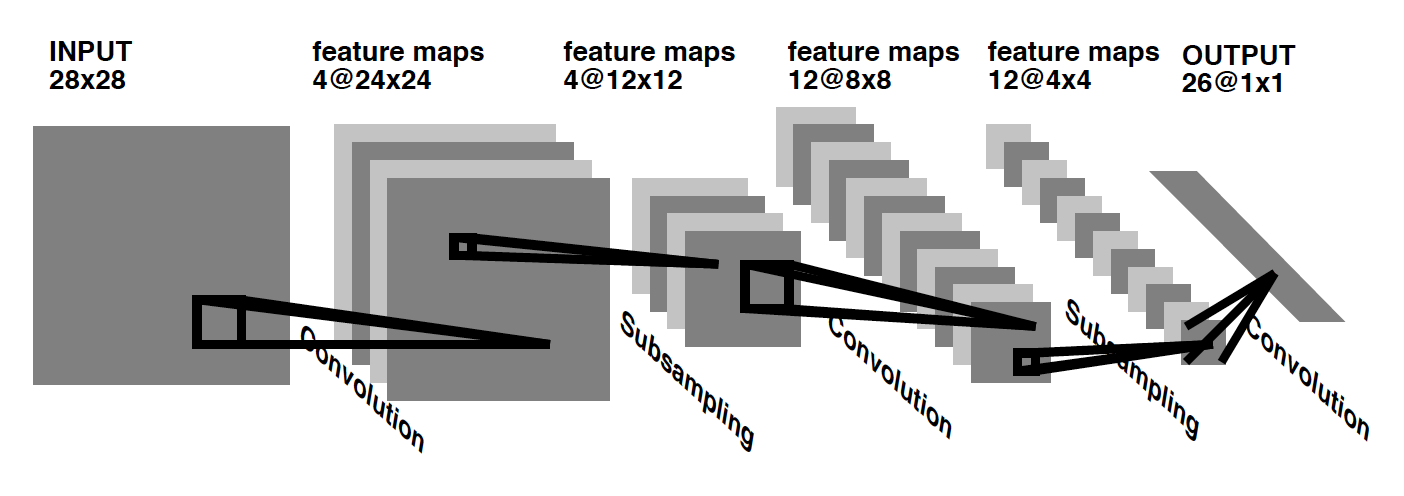
\includegraphics[width=\textwidth]{figures/CNN_architecture_LeCun}
% %  \caption{Architecture of a CNN used for classifying handwritten symbols, from \cite{LeCun95a}.}
% %  \label{fig:cnn-architecture-lecun}
% %\end{figure}

% \section{Exploratory Data Analysis}
% Exploratory data analysis (EDA) is a broad concept containing various techniques \cite{Anselin1999, Gelman2003, Hoaglin2003, Tukey1977, Velleman1981} for exploring and analysing data.
% Early popular techniques include \emph{boxplots} and \emph{stem-and-leaf} displays.
% A stem-and-leaf plot takes numbers and splits them into two groups.
% The first group contains the leading digit(s) and the second group contains the trailing digit(s).
% Figure \ref{fig:stem-leaf-plot} is an example of a stem-and-leaf plot with one leading and one trailing digit.
% The grouping helps when sorting batches of data and visualising important features, without losing the information of every single data point used \cite{Velleman1981}.

% \begin{figure} [h!]
%   \centering
%     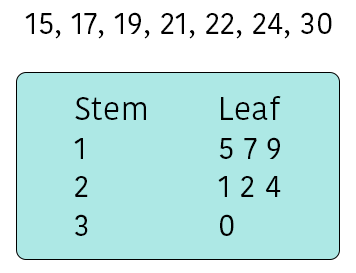
\includegraphics[width=0.33\textwidth]{figures/stem-leaf-plot}
%   \caption{Example of a stem-and-leaf plot. The numbers above the plot is the input.
%   The first digit of the number is the \emph{stem}, the following digits are the \emph{leafs}.}
%   \label{fig:stem-leaf-plot}
% \end{figure}

% \newpage
% EDA can be seen as applying tools and statistics to analyse data in a \emph{meaningful} way.
% EDA could be applied to the detection of outliers, smoothing the data, and performing a variance analysis \cite{Anselin1999, Hoaglin2003, Tukey1977, Velleman1981}.
% EDA can also reveal subtle practical problems with the chosen model that can easily be missed when performing statistical theory analysis of the model \cite{Gelman2003}.

% In \cite{Tukey1977}, Tukey describes how EDA can be used to answer research questions such as "What is the age distribution for the Vietnamese population?" and "Are there differences in
% the annual household per capita expenditures between the rural and urban populations in Vietnam?".
% Tukey uses plots to compare different groups and estimators to quantify the difference.
% For example, the sample mean estimator, or the \emph{winsorised} mean can be used \cite{Tukey1977}.
% The winsorised mean handles the case where tails of a distribution dominates the value space.  
% This would cause the sample mean estimator to poorly reflect on the "typical" data point, as it is skewed by the small tail population \cite{Tukey1977}.

% In \cite{Velleman1981}, Velleman et al. present different EDA techniques and highlights four key areas of EDA: displays (plots), residuals, re-expressions and resistance.
% Residuals is what remains after data analysis is performed.
% Residuals could, for example, be what remains after fitting data to a model (the error of the fit) \cite{Velleman1981}.
% Re-expression is the notion of applying mathematical functions to the data.
% Re-expressing the data can help with the data analysis \cite{Hoaglin2003, Velleman1981}.
% Examples of mathematical functions that can be applied are: logarithm, square root, reciprocal square function or generally raising the data to some power $p$.
% Resistance is the concept that outliers should not disproportionately affect the data analysis \cite{Hoaglin2003, Velleman1981}.
% For example, the winsorised mean estimator would be less sensitive to localised misbehaviour than the sample mean estimator \cite{Tukey1977}.

% Smoothing data is important for many different applications \cite{Bradley1997, Pang2002, Quinlan1992, Velleman1981}.
% This can, for example, be done by applying \emph{running median smoothers}.
% The running median smoothers go through all the data points in sequence and calculate only the median for the $n$ closest values near each point \cite{Velleman1981}.
% Another approach is the \emph{running weighted average} \cite{Velleman1981}.
% Instead of taking the median of the $n$ values, the average is calculated.
% The average can also be weighted with different functions, like hanning smoothing \cite{Velleman1981}.
% The hanning smoothing for three data points is shown in Eq. \ref{eq:hanning}.
% It is worth noting that a single outlier will heavily affect the hanning smoothing \cite{Velleman1981}.
% In practice it is common to first do running median smoothing to remove outliers and then apply hanning smoothing \cite{Velleman1981}.

% \begin{equation}
%   \hat y_t = \frac{1}{4} y_{t-1} + \frac{1}{2} y_t + \frac{1}{4} y_{t + 1} 
%   \label{eq:hanning}
% \end{equation}

% \section{Evaluation Metrics}
% \label{sec:eval-metrics}
% Different metrics exist for evaluating machine learning technologies.
% Common metrics are, for example, precision (Eq. \ref{eq:precision}), accuracy (Eq. \ref{eq:accuracy}), recall (Eq. \ref{eq:recall}) and F-score (Eq. \ref{eq:f-score}).
% These metrics typically use the number of true positives (TP), false positives (FP), true negatives (TN) and false negatives (FN).

% \begin{equation}
%   PRE = \frac{TP}{TP + FP}
%   \label{eq:precision}
% \end{equation}

% \begin{equation}
%   ACC = \frac{TP + TN}{P + N}
%   \label{eq:accuracy}
% \end{equation}

% \begin{equation}
%   REC = \frac{TP}{TP + FN)}
%   \label{eq:recall}
% \end{equation}

% \begin{equation}
%   F_1 = 2 * \frac{PRE * REC}{PRE + REC} 
%   \label{eq:f-score}
% \end{equation}

% \newpage
% \subsection{Cross-Entropy}
% In some contexts, e.g., in \cite{Caruana2006}, the cross-entropy is used as a metric.
% Eq. \ref{eq:cross-entropy} is the definition for the discrete case \cite{Shore1980}.
% $p$ and $q$ are two different probability distributions.
% If the output from a classifier is a probability distribution, then it would be suitable to evaluate the distribution against the "true" distribution.
% The cross-entropy function would in this case be a metric of how well the posterior distribution from the classifier performs.

% \begin{equation}
%   H(p,q) =-\sum _{x}p(x) \log q(x)
%   \label{eq:cross-entropy}
% \end{equation}

% \subsection{Machine Learning Parameters}
% Parameters for machine learning algorithms are typically chosen using cross-validation.
% First, the training data is split into $k$ sets.
% The model chooses a parameter value and trains on $k-1$ sets.
% The last set is used to evaluate the trained model, thus evaluating the chosen parameter value.
% The model that performs best according to some metric, typically accuracy \cite{Kohavi1995}, is chosen as the final model.
